\section{Introduction}
\label{sec:intro}

Creating a Geant4 simulation application devoid of hardcoded numbers can be achieved
by replacing conventional calls like ~\verb|G4Box(‘box’, 20, 30, 40)| with
code like~\verb|G4Box(name, a, b, c)| where the parameters are sourced from a database.
This however does not eliminate the need for users to write in C++ and Geant4 code
and engage in the essential tasks of organizing the volumes, specify sensitivities,
formulating the digitization of Geant4 steps, and collecting and saving the resulting hits.


\begin{figure}[h]
    \centering
    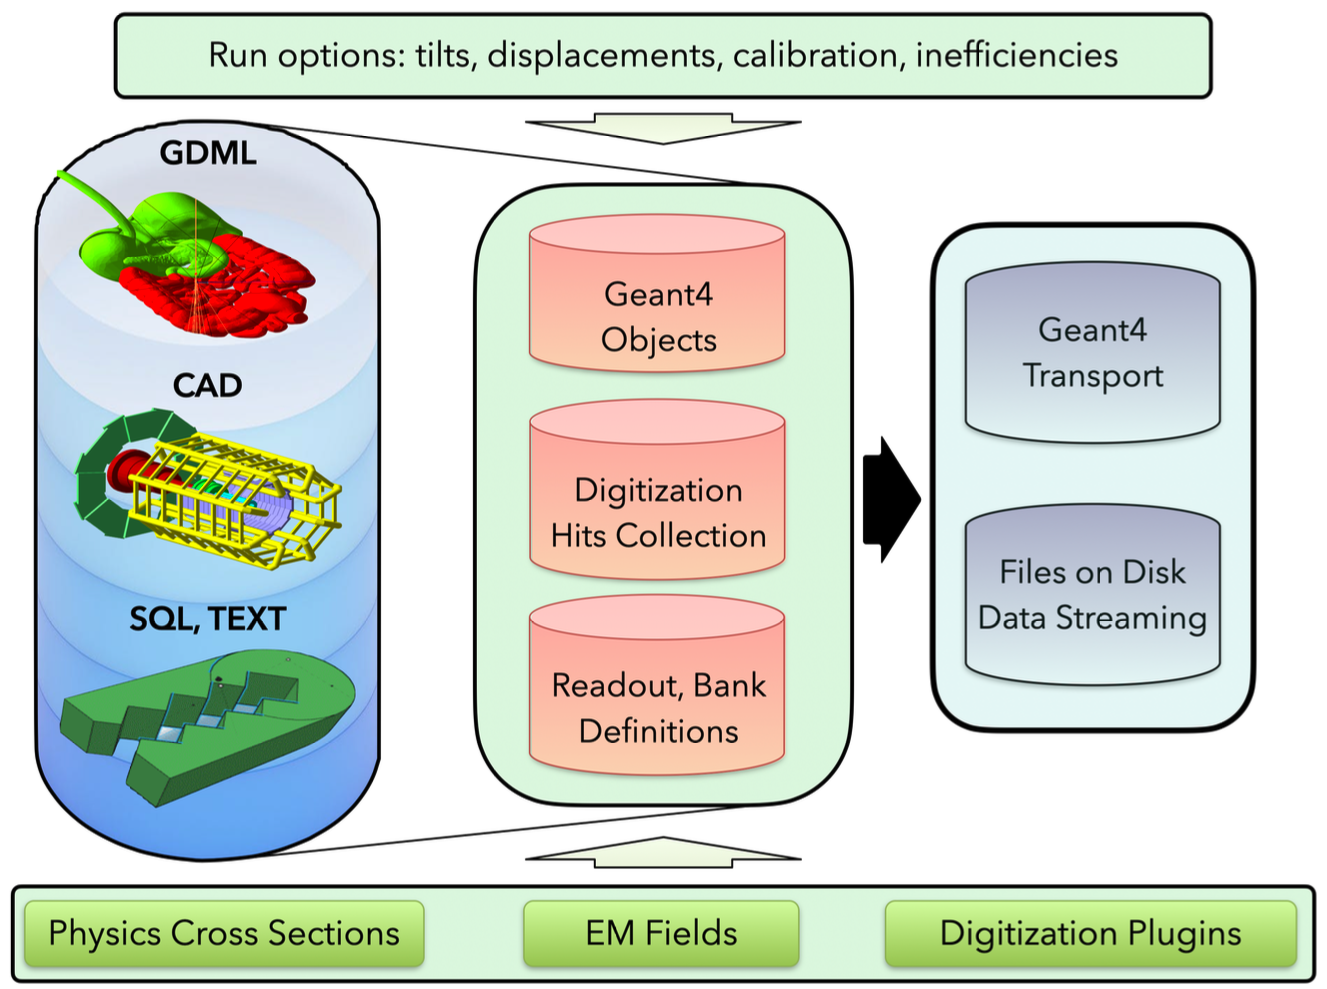
\includegraphics[width=.95\textwidth]{img/db}
    \caption{GEMC: a Geant4 application driven in its entirety by databases: geometry, materials,
        digitization, readout electronics, output format. Additional configurations such the choice
        of physics list, magnetic field, experiment setup can be provided by steering cards (JSON).}
    \label{fig:db}
\end{figure}

An application such as the one sketched Fig.\ref{fig:db}, capable of driving in its entirety
a Geant4 simulation from databases and steering cards present several advantages:

\begin{itemize}
    \item No need for prior expertise in C++ or Geant4.
    \item The focus squarely shifts towards
    the geometry aspect, facilitated by seamless interactions with databases,
    allowing users to concentrate on experiment-specific details without the burden of coding intricacies.
    \item The experiment setup is effortlessly shared without necessitating code recompilation.
    This agility enhances teamwork, limits debugging and accelerates development.
    \item It serves as a unified platform capable of simulating diverse experiments.
    Users can readily switch between experiments by selecting their desired configurations from the database.
\end{itemize}

\newpage
We present the database driven GEMC\cite{clas12_gemc, gemc_homepage}, a versatile solution that offers:

\begin{itemize}
    \item Intuitive Python API: GEMC empowers users with an accessible Python API, enabling
    effortless detector construction and seamless database population.
    Additionally, it supports Computer-Aided Design (CAD (via \emph{Stereo-lithography STL}\footnote{STL: A widely used file format
    in 3D design printing. STL represents 3D surfaces as a collection of
    interconnected triangles} files) and GDML imports, further simplifying the setup process.
    \item Hardware Emulation: GEMC incorporates hardware emulation for readout electronics.
    This allows users to mimic real-world electronic components, enhancing the accuracy and realism of
    the simulations.
    \item Custom Digitization: the flexibility to define custom digitization procedures for Geant4 steps
    ensures that the simulated detectors response mimic the real detectors'.
    \item Data Streaming: downstream analysis is facilitated by the options to stream simulation results directly
    to disk storage or network.
    Pre-loaded plugins provide ROOT and TEXT output formats.
\end{itemize}


\section{Features}
\label{sec:features}

\subsection{Geometry Sources}
\label{subsec:databases}
GEMC offers multiple sources for reading geometry and materials definitions,

\begin{itemize}
    \item CAD Import (STL): objects are defined using STL files, loaded via
    steering cards.
    Optional JSON files can add attributes like materials,
    hierarchy, position, rotation, etc.
    \item GDML files: same as CAD import, but the geometry is defined
    in a GDML file.
    \item Databases and Text Files: native Geant4 geometry and materials can be defined
    using Python API and stored in databases (MySQL, Sqlite) or text files.
    This includes combining volumes through copy and boolean operations.
\end{itemize}
Users may define volume hierarchies mixing sources.
For instance, a CAD file can be imported and serve as the parent for a volume
defined in a database, or vice versa.
This versatility empowers users to create complex geometries with ease.

\subsection{Python API}
\label{subsec:api}
Designed with a user-centric approach, the API prioritizes intuition and simplicity,
requiring no additional code beyond its usage to develop a comprehensive simulation.
In Fig.\ref{fig:api}, an example demonstrating the simplicity of the Python API to build
a detector and populate the databases is shown.
Notice how users need only to fill entries with
quantities they are familiar with, such as shape type, dimensions, etc, and not
worry about the code necessary to define the geant4 objects, assign sensitivity to the
scintillator, collect hits and writing the output.

\begin{figure}[h]
    \centering
    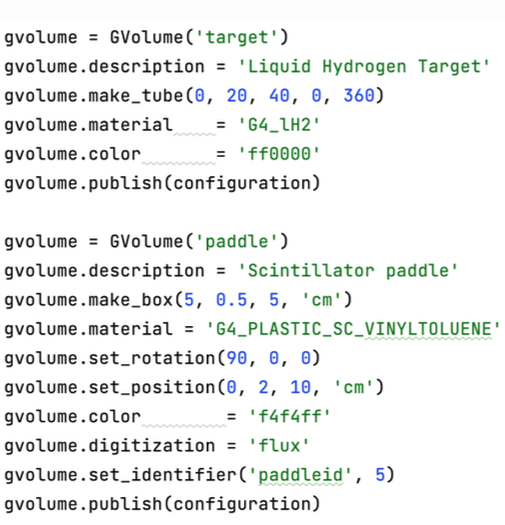
\includegraphics[width=.40\textwidth]{img/api_snippet}
    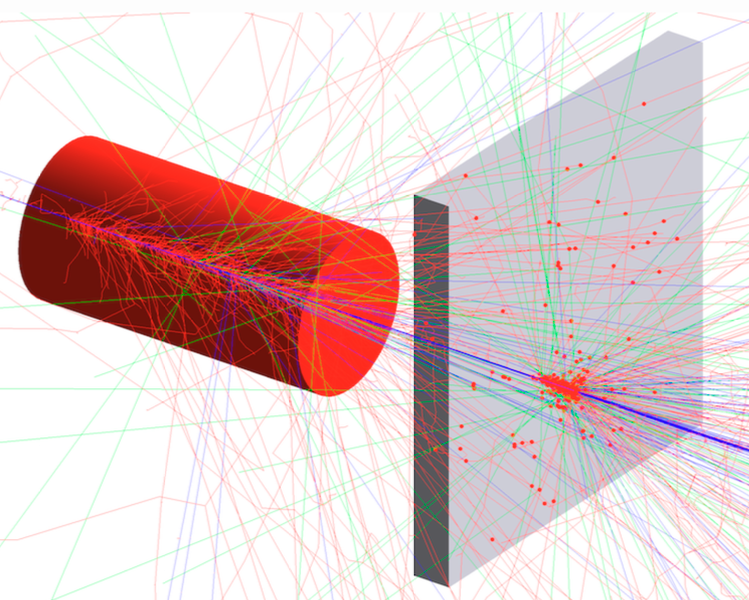
\includegraphics[width=.58\textwidth]{img/api}
    \caption{
        Left: the code snippet creates a cylindrical target and a sensitive flux box scintillator.
        Right: the resulting geometry. The flux scintillator paddle collects hits from proton
        impinging on the liquid hydrogen target.}
    \label{fig:api}
\end{figure}

The API is also used to define materials.
An example of defining a material using the fractional
mass of its constituents is shown in the code below.
Similar code is used for molecular composition and
composition with different materials

\begin{pycode}
gmaterial = GMaterial("my_peek")
gmaterial.description = "peek plastic 1.31 g/cm3"
gmaterial.density = 1.31
gmaterial.addMaterialWithFractionalMass("G4_C", 0.76)
gmaterial.addMaterialWithFractionalMass("G4_H", 0.08)
gmaterial.addMaterialWithFractionalMass("G4_O", 0.16)
gmaterial.publish(configuration)
\end{pycode}

\subsection{Electronic Time Window and Energy Sharing}
\label{subsec:time_window}

Replicating the data collection mechanism is essential to ensure that a simulation is
indistinguishable from real experimental data.
In GEMC, the integration of this critical aspect for sensitive detectors is seamless and user-friendly.

The collection of digitized values, such as integers (ADC, TDC\footnote{ADC:Analog-to-digital converter
; TDC: Time-to-digital converter. These system convert analog signals to digital signals.})
or payloads (FADC\footnote{Flash ADC: provides instantaneus conversion of analog signals to digital signals,
which enables the sampling of the shape of the signals}), within a user-set time window is handled automatically by GEMC,
see Fig.\ref{fig:time_window_energy_sharing} (left).

Furthermore, GEMC offers the capability to artificially generate hits, mimicking the phenomenon of
energy sharing commonly observed in real detectors, especially among adjacent sensitive elements like silicon strips.
The realism of simulations is enhanced by simulating energy distribution and sharing patterns
that occur naturally in experimental setups.
In Fig.\ref{fig:time_window_energy_sharing} (left) the hit
time window definition is shown: two primary tracks and a secondary track deposit energy within
the sensitive element ``cell 2''.
The triangular steps associated with the secondary track
exhibit a significant time difference compared to the circular steps, exceeding the sensitive time window.
As a result, GEMC correctly produces two separate hits, collecting the circles into one and the triangles
in the other one, mirroring the behavior of realistic readout electronics.
In Fig.\ref{fig:time_window_energy_sharing} (right) the energy sharing mechanism, a common phenomenon in real detectors,
is illustrated: the red steps are artificially generated, with a user-defined algorithm, based on the real Geant4 steps,
to mimic energy sharing.

\begin{figure}[h]
    \centering
    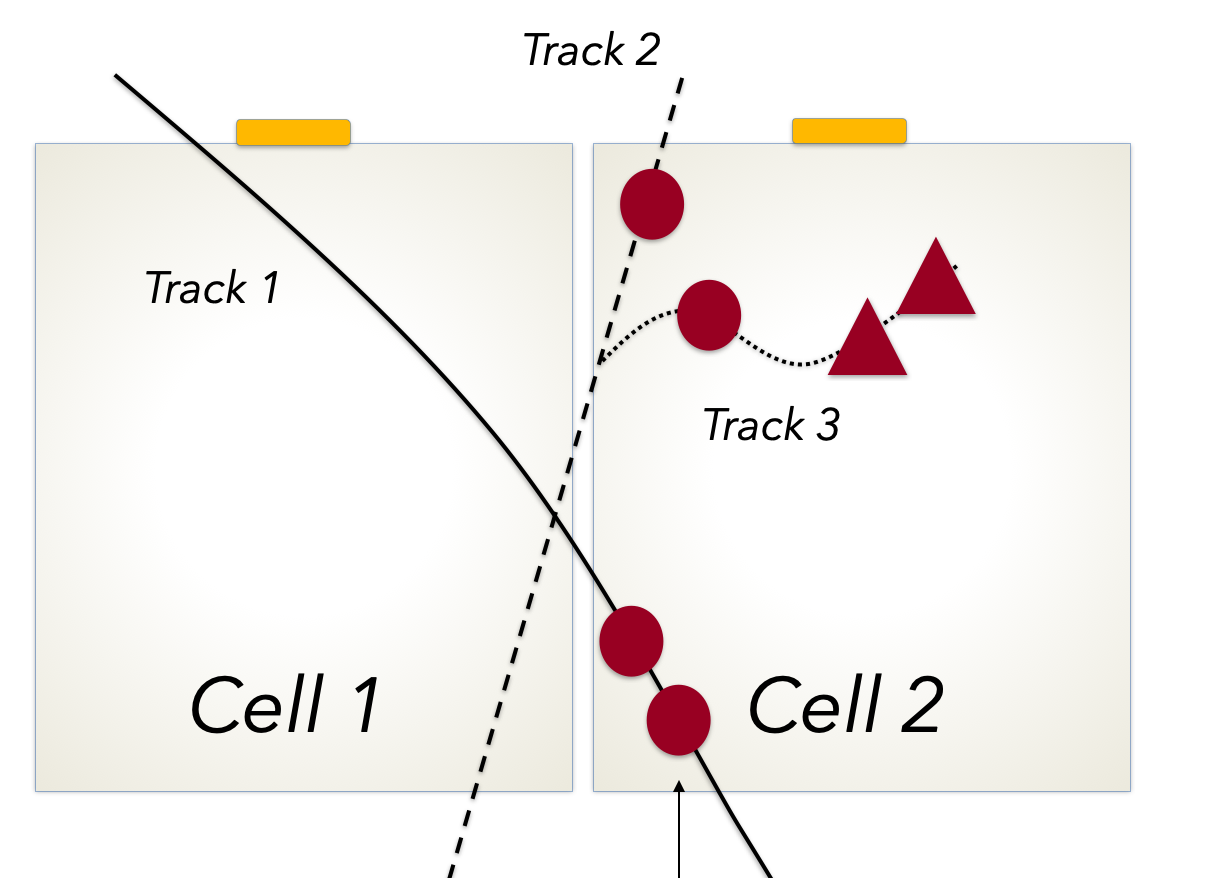
\includegraphics[width=.45\textwidth]{img/tw}
    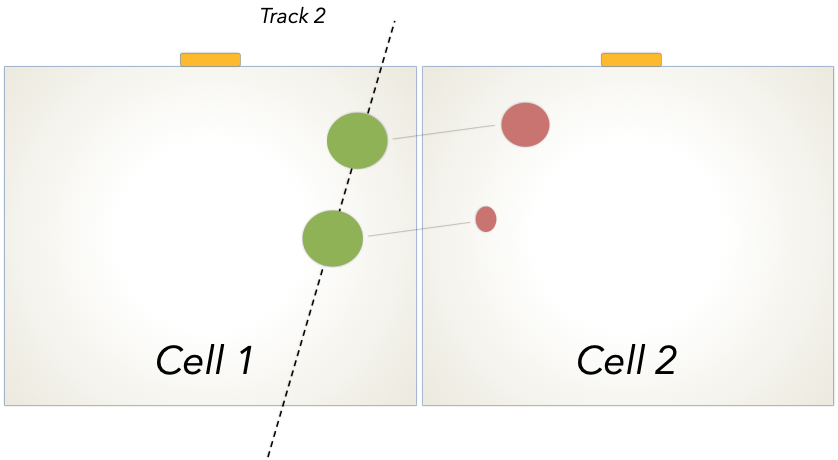
\includegraphics[width=.54\textwidth]{img/e_sharing}
    \caption{Left: the time window mechanism separates the circle and triangle Geant4 steps are collected in two hits.
    Right: the red steps are artificially generated
    to mimic energy sharing based on the green Geant4 steps.}
    \label{fig:time_window_energy_sharing}
\end{figure}

\subsection{Sensitivity and Digitization}
\label{subsec:digitization}

The digitization of Geant4 steps is a pivotal aspect of the simulation process.
GEMC simplifies this critical step by offering an intuitive interface that presents Geant4 steps
with commonly used algorithms.
Here is an overview of the functionalities it supports:

\begin{itemize}
    \item Readout Electronics Parameters: define parameters such as the time window,
    aligning simulations with real-world data acquisition.
    \item Energy Sharing and Hit Proliferation: customize energy sharing and hit proliferation mechanism.
    \item Calibration and Digitization Constants: load parameters from databases sources.
    \item Translation Table: map Geant4 volume identifiers to crate/slot/channel.
    \item Hit Digitization: collection and treatment of Geant4 steps.
    \item Streaming Readout: define parameters for data streaming to disk or network storage.
    \item Output Bank: specify the output organization for hits, such as ADC, TDC, FADC, or SRO
    payload\footnote{SRO: Streaming Readout Output. Instead of writing digital signals on disk, the
    snapshots of the readout electronics are continuosly streamed to data handlers that filter the
    data before writing it to disk}.
\end{itemize}

GEMC's plugin framework streamlines the digitization process, allowing users to tailor simulations
to closely match real-world data acquisition systems while maintaining flexibility and ease of use.

\subsection{Data Streamer}
\label{subsec:data_streamer}

GEMC provides Data Streamers to handle the storage of data to files or disk.
These streamers are stored in dynamic libraries, separate from the GEMC core, ensuring modularity
and maintainability and allowing users to create their own streamers.

They offer structured access to data collection classes like GEventDataCollection (for event-by-event hits)
and GFrameDataCollection (for time-based hits).
These streamers support a wide array of formats, including general ones like TEXT and ROOT,
as well as Jefferson Lab-specific formats like HIPO, EVIO, and VTP Binary.
This workflow simplifies data publishing, allowing users to concentrate solely on defining the variables to be
added to the data collection without concerning themselves with the intricacies of the output format.


\section{Examples}
\label{sec:examples}

Two GEMC examples that showcase its versatility and practicality are shown.
The first illustrates the CAD integration.
The second example takes us to the CLAS12 experiment at Jefferson Lab, where GEMC plays the role
of simulating and calculating the response of real-world experiments and data acquisition processes.

\subsection{Cad Import}
\label{subsec:cad_import}

This example highlights GEMC's versatility in handling CAD imports and its ability to create engaging
simulations of complex scenarios with minimal coding.
The goal is to visualize and simulate interactions between two iconic spacecraft: an Enterprise ship and a Romulan ship.

\begin{figure}[h]
    \centering
    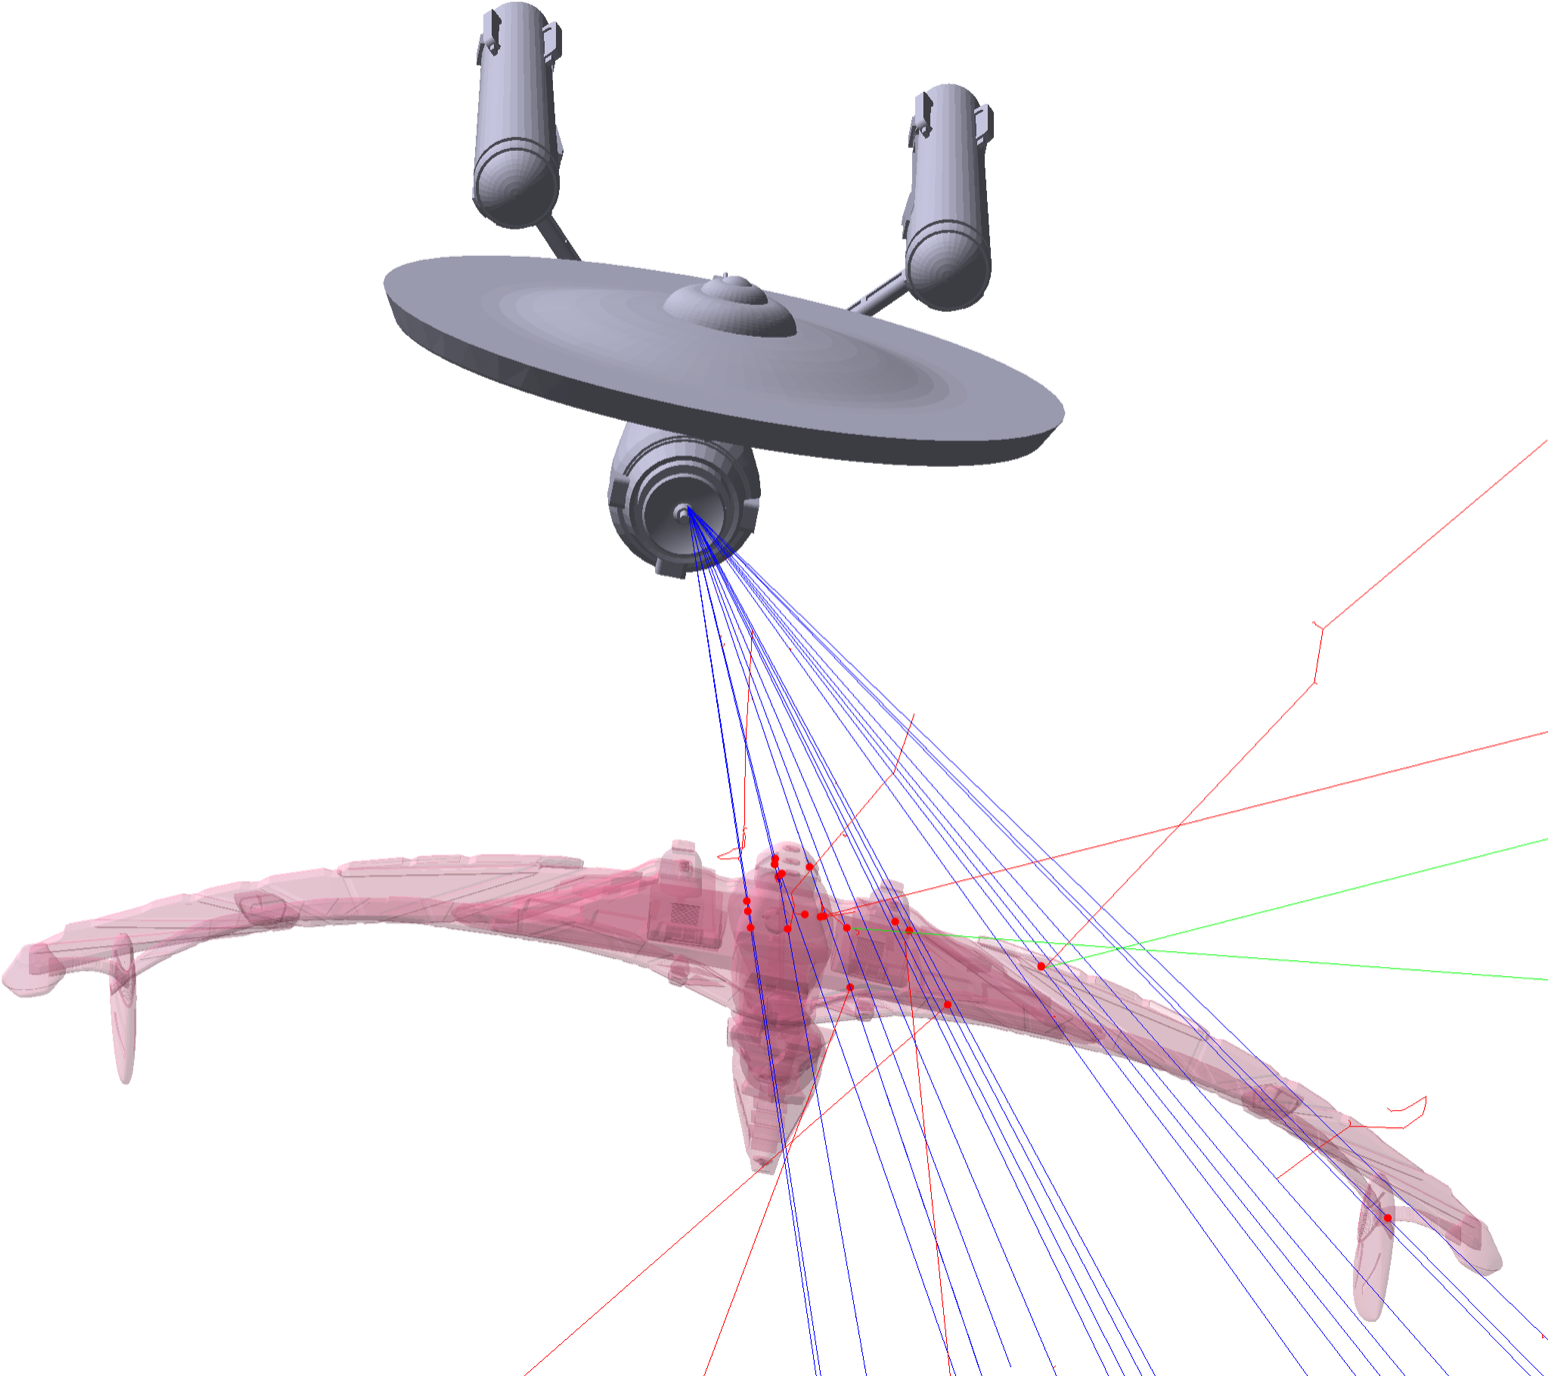
\includegraphics[width=.5\textwidth, height=0.2\textheight]{img/startrek}
    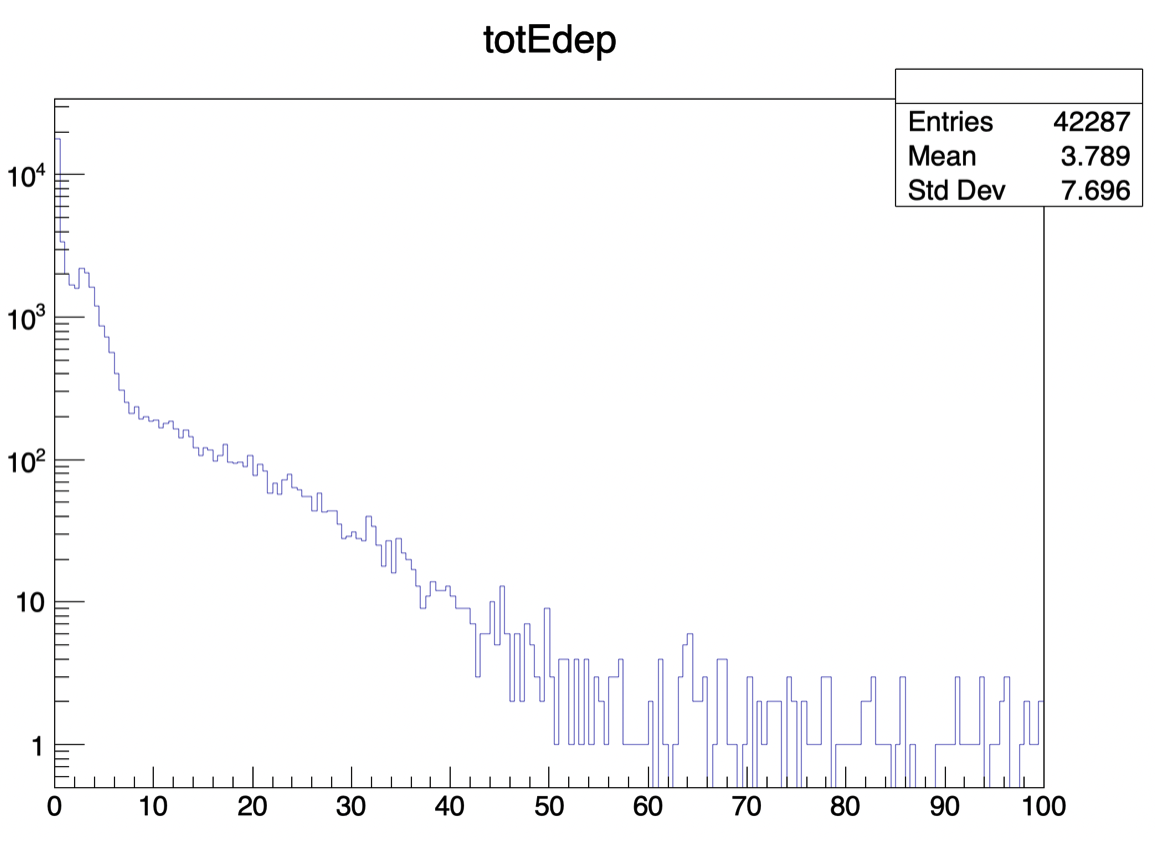
\includegraphics[width=.48\textwidth]{img/startrek_edep}
    \caption{Left: the geometry of the Enterprise and Romulan ships imported from STL files.
    A proton beam is shot at the Romulan ship and the resulting energy deposited in the Romulan ship
    is shown to the right.}
    \label{fig:cad_import}
\end{figure}


The volumes are imported directly from two STL
files: ``enterprise.stl'' and ``romulan.stl''.
The following line in a JSON steering card takes care of the romulan ship color, including its transparency that honors the cloaking technology,
and assigns the ``flux'' sensitivity to it:

\begin{verbatim}
"romulans": {"color": "ff99bb4", "digitization": "flux"}
\end{verbatim}

With command line options a proton beam is shot at the Romulan ship.
No actual code is required to run the simulation, shown in Fig.\ref{fig:cad_import}.

\subsection{GEMC at Jefferson Lab}
\label{subsec:clas12}
GEMC is used for simulations of the CLAS12 (CEBAF Large Acceptance Spectrometer
for operation at 12 GeV beam energy)~\cite{clas12_gemc} spectrometer at the Thomas Jefferson National
Accelerator Facility.
CLAS12 is designed to study electro-induced nuclear and hadronic reactions
by efficiently detecting charged and neutral particles over a large solid angle.
It consists of two superconducting magnets and multiple detector subsystems.
These detectors include Drift Chambers, Cherenkov Counters, Ring-Imaging Cherenkov Counters,
central and forward time-of-flights (CTOF, FTOF), forward trackers (FT) and electromagnetic calorimeters,
silicon vertex trackers (SVT) and more.

The geometry and materials, stored in databases, are a combination of native Geant4 volumes and
CAD imports.
In Fig.\ref{fig:clas12}, a few components are shown.
In particular the CLAS12 torus hardware's volumes are imported from the CAD engineering model.
Detailed in bottom left, the warm and cold hubs are visible,
along with the tungsten shielding in the innermost part of the hub.
The central detector is shown on top right: the target is surrounded by 3 layers of SVT and
6 layers of Micromegas, 3 with Z- strips, 3 with C-strips.
On the downstream end (beam incident from the left) the Forward Micromegas Tracker disks are visible.

\begin{figure}[h]
    \centering
    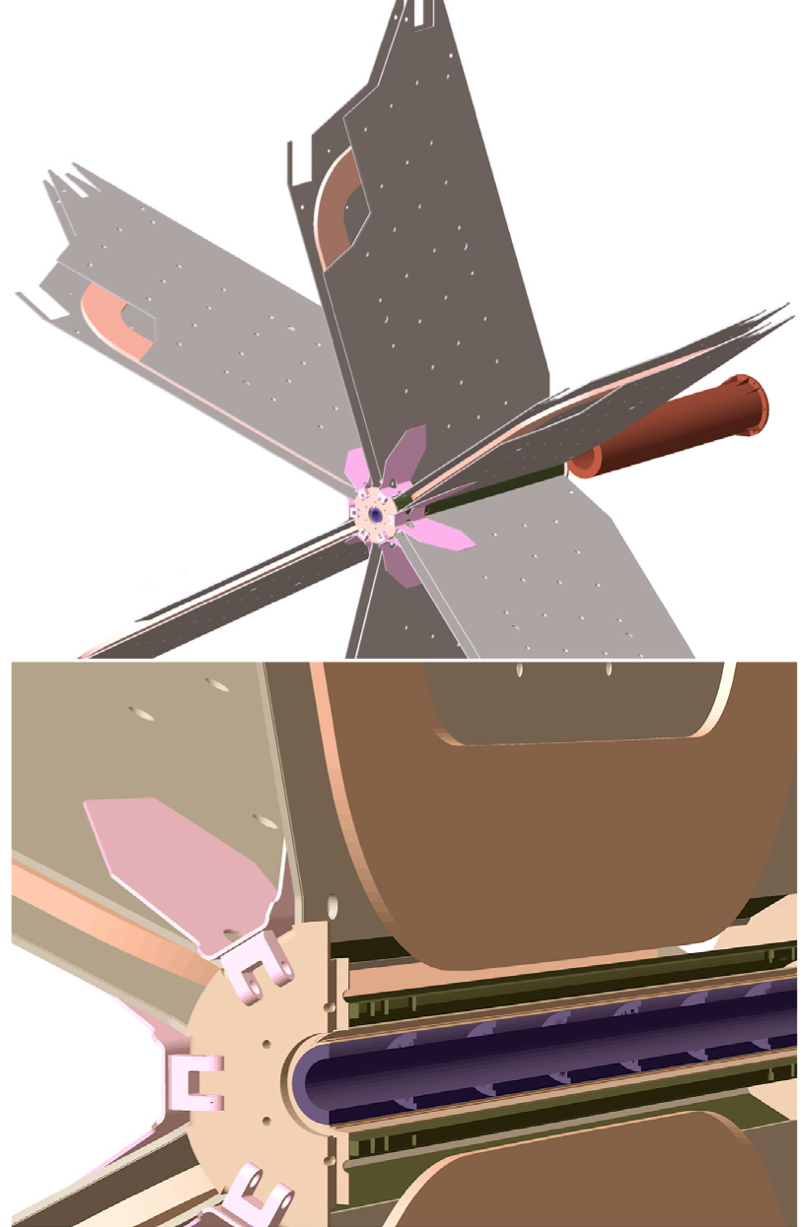
\includegraphics[width=.48\textwidth]{img/c12_torus}
    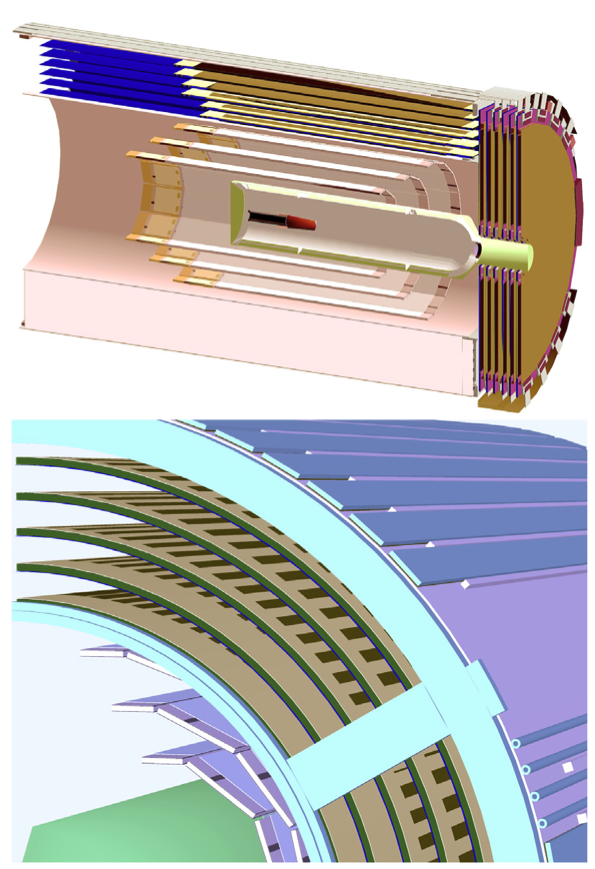
\includegraphics[width=.48\textwidth]{img/c12_ct}
    \caption{
        Top Left: the GEMC implementation of the CLAS12 torus hardware.
        Bottom Left: a section view of the torus in the vicinity of the beamline.
        Beam is incident from the left.
        Top Right: a longitudinal cut view of the CLAS12 Central Detector trackers.
        Bottom Right: detail of the Micromegas GEMC geometry, showing the overlay cover,
        the copper ground, and the PCB.}
    \label{fig:clas12}
\end{figure}

The performance of the GEMC CLAS12 simulations is evaluated by comparing the predicted background
rates from beam interactions with experimental data.
The predictions are based on the simulated interactions of the 11 GeV electron beam
with the CLAS12 target, using the various electronics time windows and thresholds
to accumulate hits in the detectors.
A typical single event of these simulations contains about 120 thousand electrons to match
the CLAS12 experimental conditions.
Examples of these studies are shown in Fig.\ref{fig:clas12_rates}, where simulations were run
at the full CLAS12 $10^{35} cm^{-2} s^{-1}$
luminosity, corresponding to 124,000 electrons in a 250 ns time window.
The scattering electrons along the beamline are focused along the beamline by the solenoid,
an effective electromagnetic shield for CLAS12.
The choice of energy threshold in the SVT
is shown in the bottom left panel: the hits are represented by the squares.
The threshold applied in the four plots are: no energy cut; 10, 20, 30 keV.
The SVT final choice of threshold based on the background rejection study was 30 keV.
The table showing the fluences and radiation doses in the SVT layers is also shown on the bottom right.

\begin{figure}[h]
    \centering
    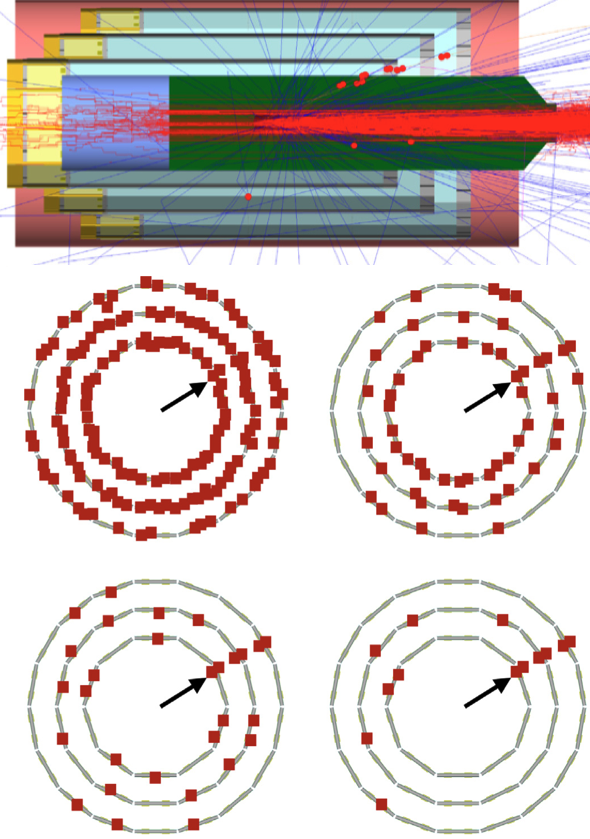
\includegraphics[width=.48\textwidth, height=0.3\textheight]{img/c12_rates}
    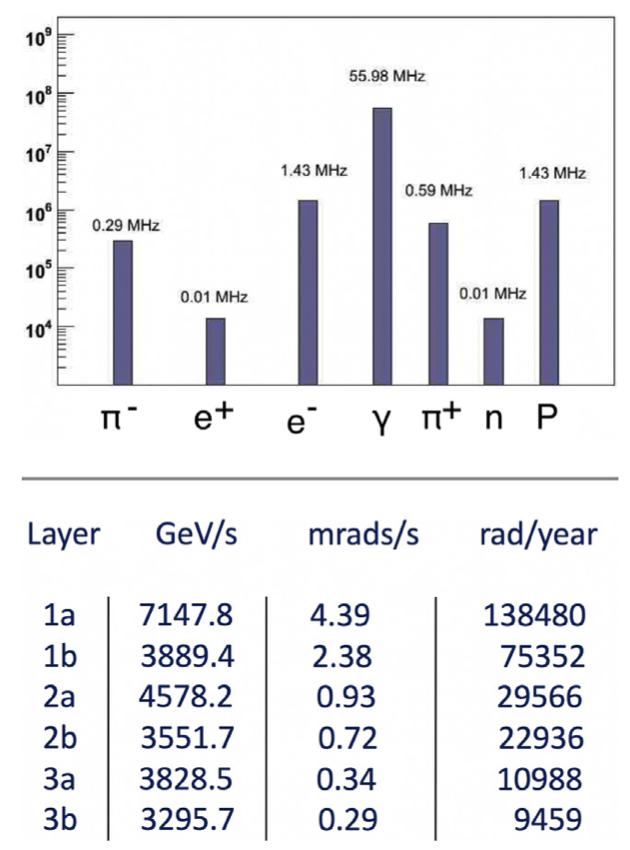
\includegraphics[width=.48\textwidth, height=0.3\textheight]{img/c12_bst}
    \caption{
        Top Left: one event in the Central Detector
        at the full CLAS12 $10^{35} cm^{-2} s^{-1}$ luminosity
        Bottom Left: The occupancy in the SVT layers for different thresholds for
        one event containing a proton track (direction indicated by the arrow).
        Right: Summary of radiation doses and background rates in the SVT.
        The rate breakdown for different particles for a threshold of 20 keV
        at the full luminosity of CLAS12.
    }
    \label{fig:clas12_rates}

\end{figure}

The nominal luminosity of $1 \times 10^{35} cm^{-2} s^{-1}$ was achieved in CLAS12 in
December 2017, and rates in each of the CLAS12 detectors were measured.
The rates in the Drift Chambers were found to be in good agreement with the GEMC predictions, see
table~\ref{tab:rates}.
Similar agreements were found with the rates in the other CLAS12 detectors.
In particular:

\begin{itemize}
    \item FTOF: good agreement with data for the PMT currents~\cite{ftof-nim}.
    \item CTOF good agreement with data for the upstream PMT counter rates, while the downstream counter rates
    are about a factor of three lower in the simulation than they are in the data, probably due to the simulation
    not taking into account the Cherenkov light produced in the light guides~\cite{ctof-nim}.
    \item FT: good agreement with data for PMT currents and radiation doses~\cite{ft-nim}.
\end{itemize}

\begin{table}[h]
    \begin{center}
        \begin{tabular}{| c | c | c |}
            \hline \hline
            Region & Data  & GEMC  \\
            \hline
            1      & 2.8\% & 2.7\% \\
            2      & 0.6\% & 0.8\% \\
            3      & 1.5\% & 1.2\% \\
            \hline \hline
        \end{tabular}
    \end{center}
    \caption{Drift chamber hit occupancy comparison between simulation and data.}
    \label{tab:rates}
\end{table}

GEMC has been shown to perform very well when comparing simulation rates to
data and it was an essential component to optimize the design of the CLAS12 detectors,
their associated calibration procedures, and their ultimate performance.


\section{Conclusion}
\label{sec:conclusion}

In conclusion, the article presents GEMC, a Geant4 simulation application
capable of creating Geant4 simulations by leveraging databases and steering cards.
It eliminates the need for users to have expertise in C++ and Geant4 coding,
allowing them to focus on experiment-specific details.

Key takeaways include GEMC's intuitive Python API, which simplifies detector
construction and database population, as well as its ability to emulate real-world
hardware, customize digitization processes, and streamline data output to disk or network.

These features empower researchers to create accurate and efficient simulations while significantly
reducing development time and coding complexities.